
\documentclass[14pt]{beamer}

\mode<presentation> {

\usetheme{Pittsburgh}
\usecolortheme{owl}
\setbeamertemplate{footline}[page number] % To replace the footer line in all slides with a simple slide count uncomment this line

\setbeamertemplate{navigation symbols}{} % To remove the navigation symbols from the bottom of all slides uncomment this line
}

\usepackage{graphicx} % Allows including images
\usepackage{subfigure}
\usepackage{soul}
\usepackage{xcolor}


\title[Short title]{Mammography breast cancer detection} 

\author{Phuc Nguyen} % Your name

\date{April 2023} % Date, can be changed to a custom date

\begin{document}

\begin{frame}
\titlepage % Print the title page as the first slide
\end{frame}


\begin{frame}{\small Problem identification}
    \begin{itemize}
        \item As many as half of women experience false positive mammography screening, leading to costly medical procedures.
        \item We would like to automate breast cancer detection using ML. \\~\
        \item Advantage: might improve false positive rate (FPR), thereby improving patient care.
    \end{itemize}
\end{frame}

\begin{frame}{\small Data Wrangling}
\begin{itemize}
    \item 
    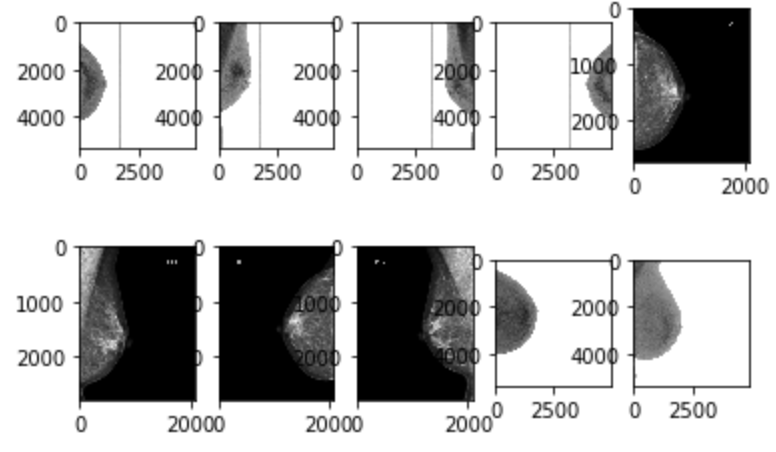
\includegraphics[width=0.75\textwidth]{RawMammograms}\\~\
    2 types of mammograms: different backgrounds, different sizes.\\~\
    \item Converted to white background, size 512 x 512.
\end{itemize}
\end{frame}

\begin{frame}{\small Data Wrangling (cont.)}
\begin{itemize}
    \item Cleaned up \colorbox{yellow}{view}:
    \begin{itemize}
        \item 'ML', 'LM', 'LMO' typos for 'MLO' (medio-lateral oblique)\\~\
        \item 'AT' deleted
    \end{itemize}

    \item Dropped rows with missing data\\~\
    
    \item One-hot encoding
    
\end{itemize}
\end{frame}

\begin{frame}{\small EDA}
\begin{itemize}
\item 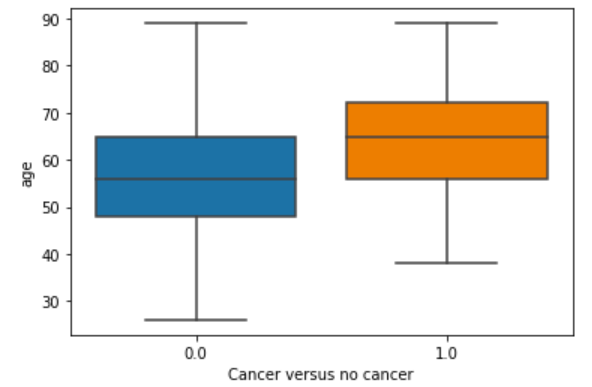
\includegraphics[width=0.75\textwidth]{AgeVsCancer}\\~\
Median \colorbox{yellow}{age} is higher among patients with cancer.
\end{itemize}
\end{frame}

\begin{frame}{\small EDA (cont.)}
\begin{itemize}
\item 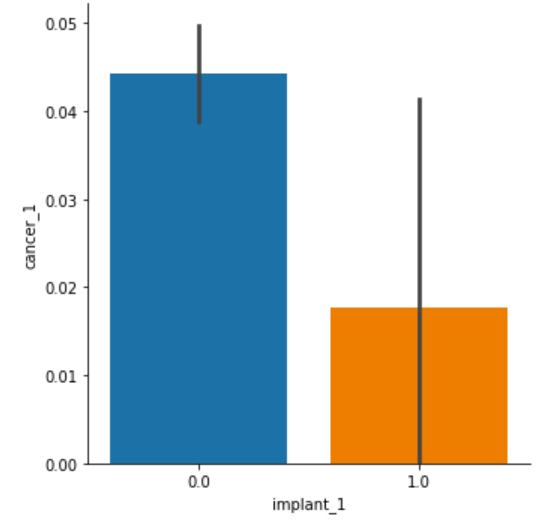
\includegraphics[width=0.5\textwidth]{CancerVsImplant}\\~\
Interestingly, cancer is less likely among patients with \colorbox{yellow}{breast\_implant} !
\end{itemize}
\end{frame}

\begin{frame}{\small EDA (cont.)}
\begin{itemize}
    \item We found the distribution of \colorbox{yellow}{breast\_density} to be:
    \begin{itemize}
        \item Density A: 10 \% of patients
        \item Density B: 43 \% of patients
        \item Density C: 42 \% of patients
        \item Density D: 5 \% of patients
    \end{itemize}
    Same as breast density distribution in the general population.
    \item Mammograms evenly distributed between \colorbox{yellow}{laterality} L (49.8 \%) and laterality R (50.2 \%)
    \item Mammograms evenly distributed between \colorbox{yellow}{view} CC (48.6 \%) and view MLO (51.4 \%)
\end{itemize}
\end{frame}

\begin{frame}{\small Preprocessing}
\begin{itemize}
    \item Feature engineering with \colorbox{blue}{HOG} (histogram of oriented gradients), instead of using pixel values directly.\\~\
    
    \item Undersampling and oversampling with \colorbox{blue}{SMOTE}.\\~\
    
    \item Scaling with \colorbox{blue}{MinMaxScaler}.\\~\
    
    \item \colorbox{blue}{PCA} transformation with 100 components.\\~\
\end{itemize}
\end{frame}

\begin{frame}{\small Preprocessing (cont.)}
\begin{itemize}
    \item 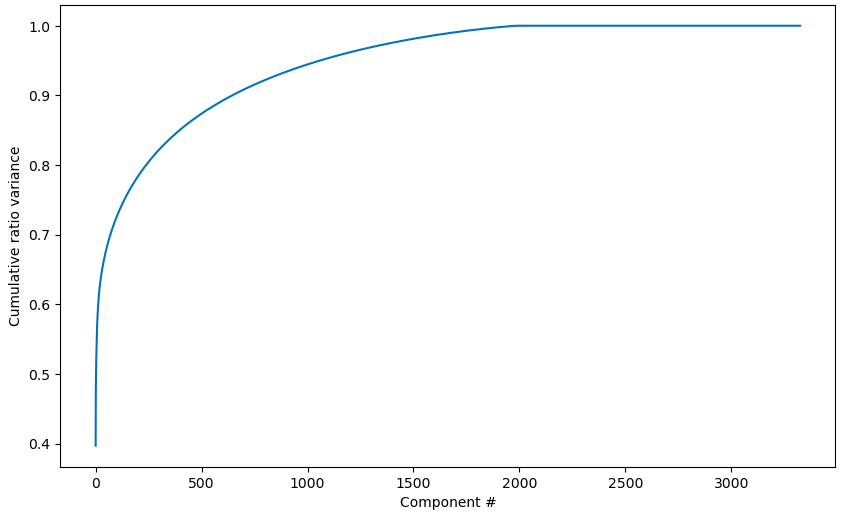
\includegraphics[width=0.75\textwidth]{PCA}\\~\
    100 PCA components explain around 0.6-0.7 of the cumulative ratio variance
\end{itemize}
\end{frame}

\begin{frame}{\small Modelling}
\begin{itemize}
    \item Trained 3 models:
    \begin{itemize}
        \item Logistic Regression\\~\
        \item Random Forest\\~\
        \item Boosted Gradient
    \end{itemize}
    \item Performance metric: F1 score.\\~\
    \item Hyperparameter search with 5-fold cross-validation.
\end{itemize}
\end{frame}

\begin{frame}{\small Modelling (cont.)}
\begin{itemize}
    \item Best model: Logreg
    \item Bayesian hyperparameter search for \colorbox{green}{C} over the range 0.01-200.\\~\
    \item F1-score on training data: 0.96\\~\
    \item F1-score on testing data: 0.64
\end{itemize}
\end{frame}

\begin{frame}{\small Modelling (cont.)}
\begin{itemize}
    \item For random forest, we did hyperparameter search for \colorbox{green}{min\_samples\_split}, \colorbox{green}{max\_depth}, \colorbox{green}{criterion}, \colorbox{green}{max\_features}, \colorbox{green}{bootstrap}. \\~\
    \item F1-score on testing data only 0.26.\\~\
    \item For gradient boosting, we did hyperparameter search for \colorbox{green}{learning\_rate}, \colorbox{green}{min\_samples\_split}, \colorbox{green}{max\_depth}, \colorbox{green}{criterion}, \colorbox{green}{max\_features}.\\~\
    \item F1-score on testing data only 0.35.
\end{itemize}
\end{frame}

\begin{frame}{\small Modelling (cont.)}
\begin{itemize}
    \item 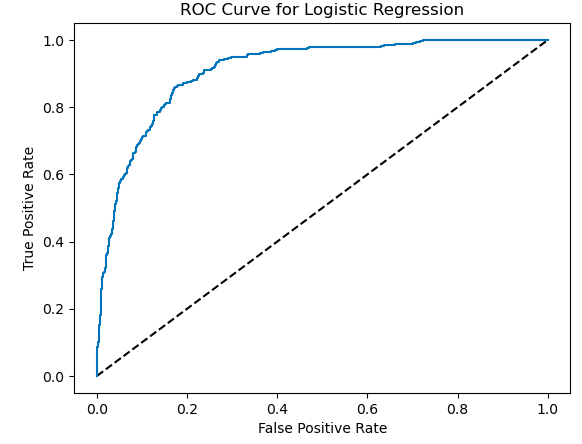
\includegraphics[width=0.75\textwidth]{LogRegROC}\\~\
    ROC-AUC for log reg: 0.91.
    \item The eblow occurs at a FPR below 0.25, which is what we want.
\end{itemize}
\end{frame}

\begin{frame}{\small Conclusion and future improvements}
\begin{itemize}
    \item By deploying the logistic regression model, we hope to bring down the FPR to below 25 percent within the next 5 years.
    \item If we had tried to use more images, Kaggle Kernel would have run out of memory. In the future, we would like to use more images.
    \item Use more PCA components ? Search hyperparameter more thoroughly ?
    \item Use neural nets ?
\end{itemize}
\end{frame}

\end{document}
